\documentclass[Report.tex]{subfiles}
\begin{document}

\chapter{Introduction}
\section{The Problem}
The last few decades have seen the availability of digital content dramatically increase, as adoption of the World Wide Web and other internet technologies became widespread both at home and in the workplace. Academic publishing was soon to capitalise on this trend, with long-established journals such as Nature creating websites for all aspects of the publishing pipeline, from submission to publication of papers online, in the '90s \cite{nature-history}. This increase in accessibility has contributed toward an exponential growth of literature \cite{hunter-cohen} that can make the search for relevant papers challenging in the present day. PubMed, a freely-available online database for medical texts maintained by the National Center for Biotechnology Information (NCBI) of the National Institutes of Health (NIH) in the United States, is a mainstay for many users in the health and academic sectors and is accessed by millions of users daily \cite{dogan}.  However, the web interface presents a simplistic approach to information retrieval, with minimal analysis of results and a relatively steep learning curve for achieving satisfactory results with text queries alone. An example of a results page can be seen in Figure \ref{fig:pubmed}. This rich source of information combined with a lack of utilities has provided the motivation for this project: to utilise the information contained within indexed citations to represent data in an information-rich and visual way.\newline

\begin{figure}[!ht]
\begin{center}
	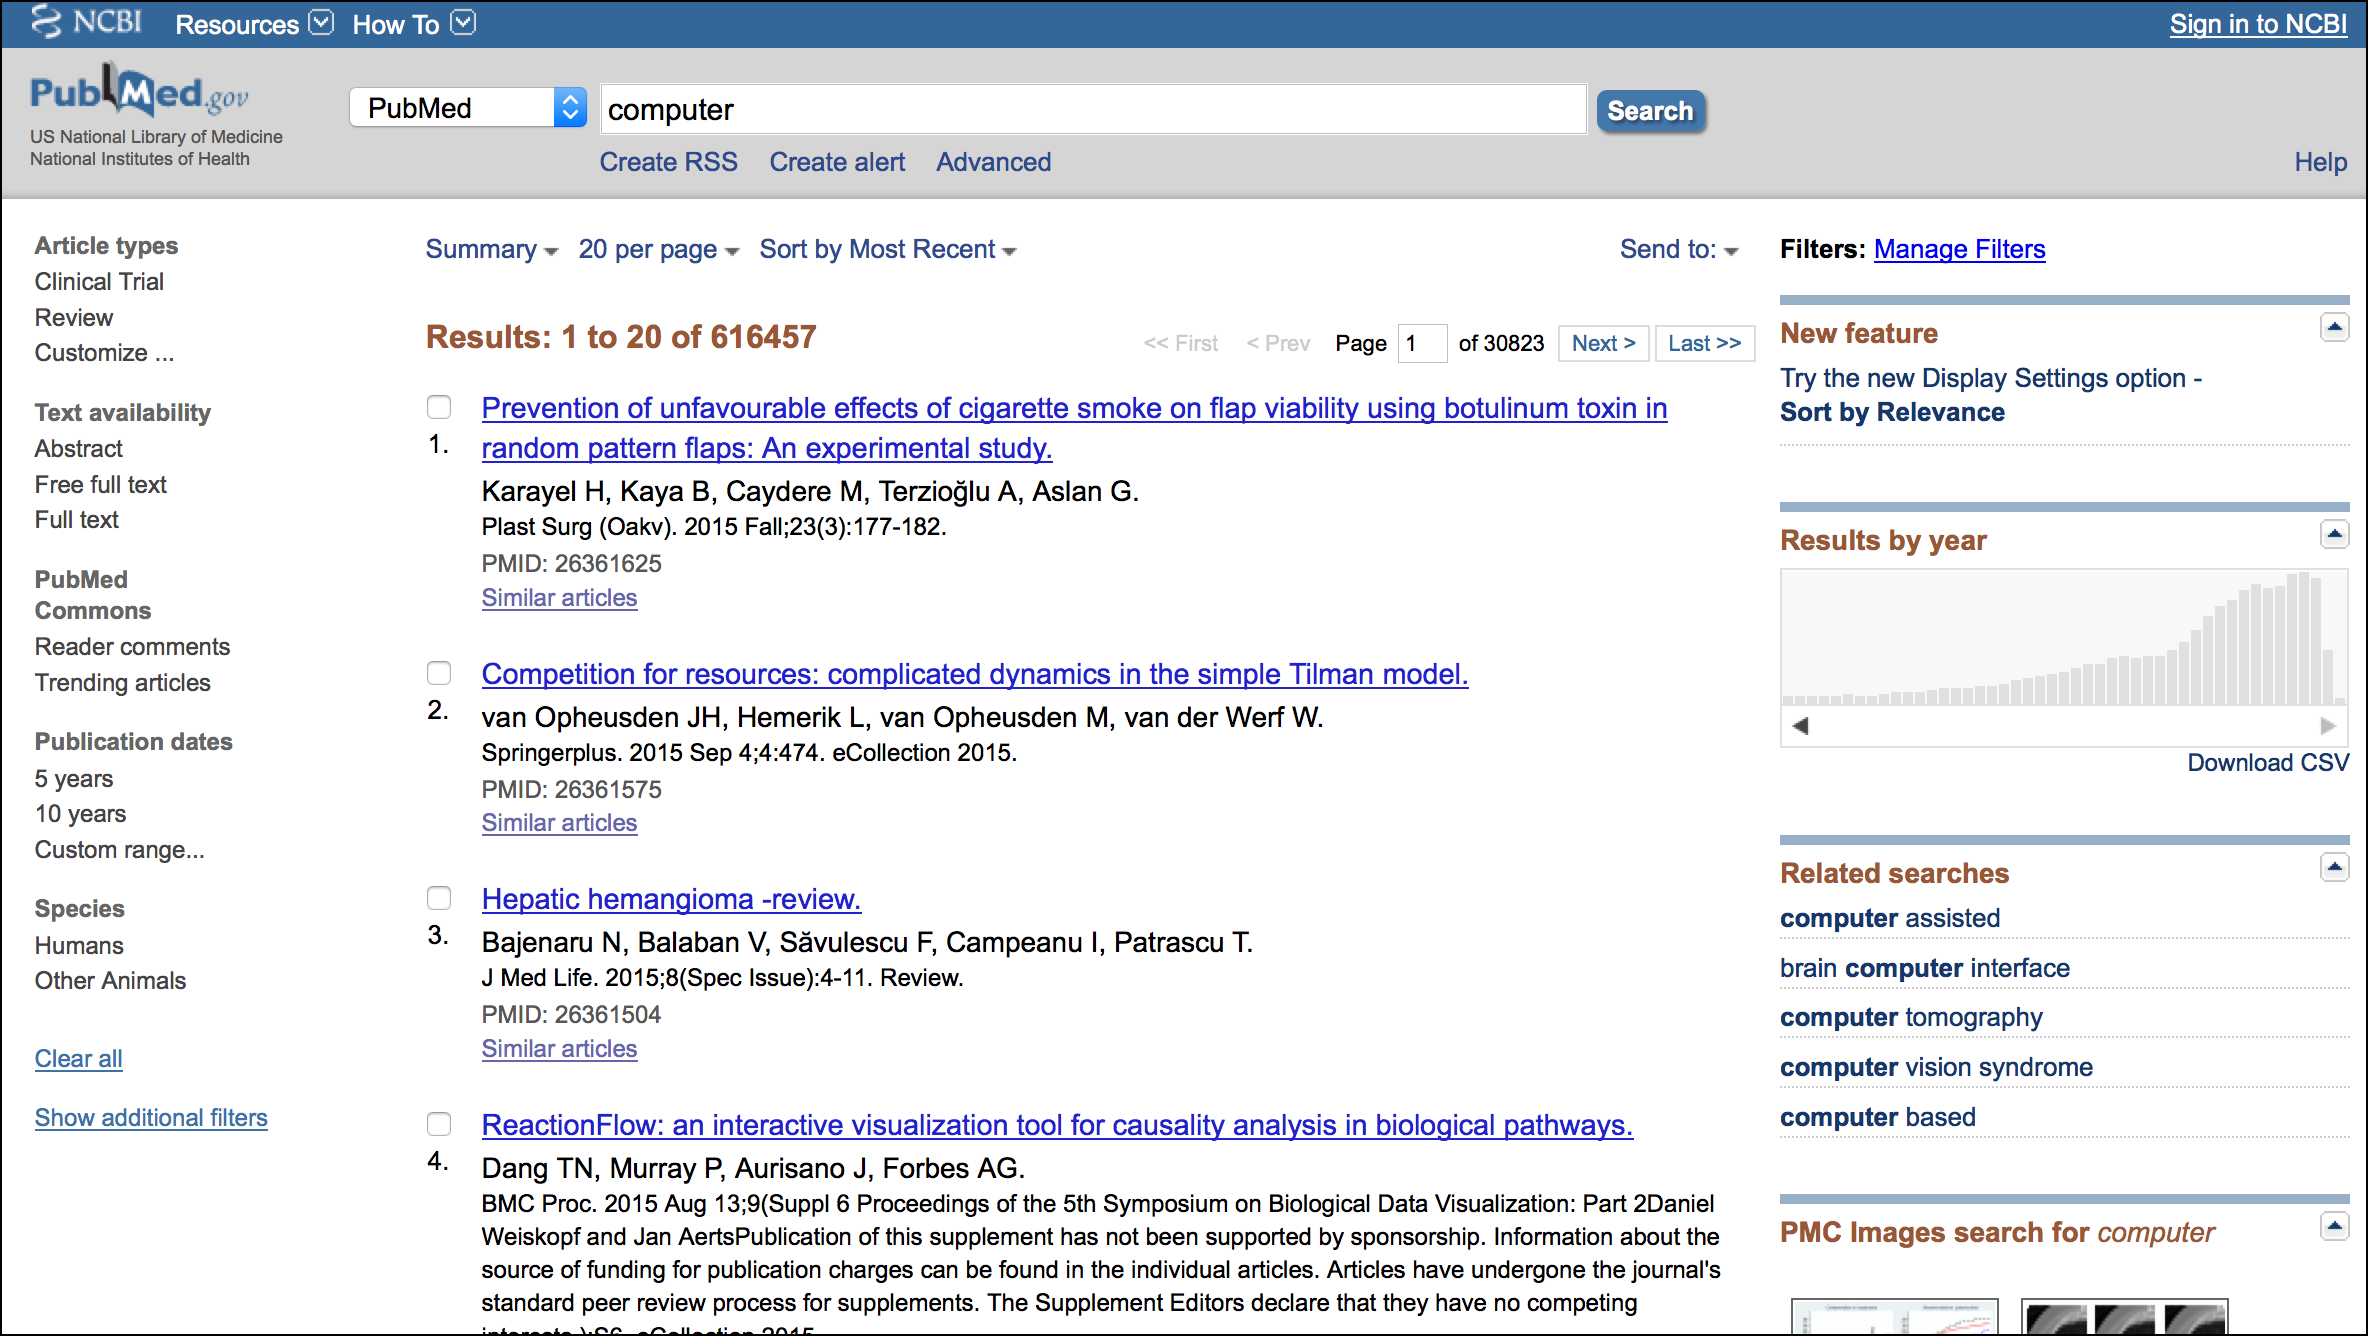
\includegraphics[width=0.8\textwidth]{../lib/images/pubmed.png}\\
	\caption{The results page of PubMed after the term 'computer' is entered.\label{fig:pubmed}}
\end{center}
\end{figure}

\section{Related Work}
A great deal of work has been carried out on the analysis and optimisation of PubMed as a service. The proposal discussed a small number of web applications that allow users to view citations in different ways, such as through the generation of static graphs with GoPubMed \cite{gopubmed}, or by creating a social network-like web application for authors with Microsoft Academic Search \cite{mas}. Of note, GoPubMed implements a text recognition algorithm in order to extract terms that are known to belong to a specific hierarchical vocabulary, the Gene Ontology. This definition of text in terms of real-world concepts is known as word-sense disambiguation (WSD). Citations are indexed with relationships to these terms, allowing efficient retrieval upon the execution of a relevant query. To my knowledge, GoPubMed does not disambiguate terms, which may result in a lower success rate of assigning vocabulary entries to papers. Natural language processing and WSD are particularly challenging in biomedical literature, as multiple nomenclatures can exist for the same concept, such as with Latin and colloquial names (humans vs. \emph{Homo Sapiens}), chemical names (water vs. H{\textsubscript{2}}O) and acronyms (Polymerase Chain Reaction vs. PCR).\newline

\noindent MetaMap, developed by Alan Aronson at the NIH, is able to disambiguate strings to a single concept present in the Unified Medical Language System (UMLS) based on other terms found in the same sentence or block of text \cite{metamap2000}. MetaMap can also be used to categorise documents, enabling users or developers to create filters to narrow down search results. This approach was adopted by Li and Zu \cite{lizu} to develop an automated alternative to human curation of medical literature. In their methodology, PubMed user logs were analysed to obtain a set of citations that were then sorted according to relevance of the topic of interest, as determined by the concepts returned by MetaMap. This approach tackles the problem of excessive search results from the ground up: it builds upon past user data to inform future user behaviour. The neatness of this approach is acknowledged, though there are concerns of creating a search 'bubble' - for example if a citation is missed by MetaMap, it will then be missed by a large number of users due to its exclusion from the topic filter. The filters would require updating to incorporate more recent user logs, but may then exclude unpopular, but potentially relevant, citations. The strategy of this project is to instead provide users with extra information, leaving the filtering behaviour to be carried out manually. 

\section{Relevant Technologies}
The main strength of this application is its ability to integrate information from various sources to produce enriched data points. Each of these services fills a specific role in the pipeline, eventually resulting in a citation that has associated with it a list of concepts from the UMLS as well as geographical coordinates corresponding to the institutions that the authors are affiliated with. The external systems are introduced here, as they are referred to throughout the report.

\subsection{NCBI E-Utils}
PubMed is accessible through a RESTful web service provided by the NCBI as part of their Entrez utilities interface (referred to as 'E-Utils') \cite{eutils}. Between them, the Entrez databases index genome sequences, taxonomies and full-text articles, as well as the citations and abstracts in PubMed. Literature comprising PubMed includes conference proceedings, journal articles, book chapters and newsletters. PubMed can be searched much in the same way as with the web interface (available at \url{http://www.ncbi.nlm.nih.gov/pubmed/}) by entering a text query with a possible match to any field in the bibliographic information (such as the title, authors and journal the article was published in) or in the abstract. If any matches are found, the E-Utils return results in either XML or JSON format. 

\subsection{MetaMap, MTI and the UMLS}
As mentioned above, MetaMap is a specialised piece of natural language processing software for detecting medical concepts in texts. It was developed in order to fully utilise the UMLS for data mining, information retrieval and indexing citations \cite{metamap2000}. In brief, MetaMap works by tagging and extracting short phrases of primarily nouns and verbs from the input text, that are then compared against a vocabulary to check for synonyms and abbreviations. Any matching terms are retrieved after analysis of any ambiguity or over-matching. The hierarchical and non-hierarchical relationships are represented in the MetaThesaurus, a relational dataset of concepts that consists of up to 150 specialist vocabularies in the biomedical domain. Though MetaMap uses the MetaThesaurus to analyse the concepts and determine which are most appropriate, the relationships themselves do not form part of the output. MetaMap is configurable if, for example, the input is a list of known terms or the sensitivity of the mapping algorithm needs to be increased \cite{metamap2010}. MetaMap is part of a larger system provided by the NIH, called the Medical Text Indexer (MTI) \cite{mti}. In this pipeline, UMLS concepts are extracted using MetaMap, clustered, and then ranked. The MTI also searches a database to find neighbouring citations and thus find common concepts between these. This approach that gleans information external to the data from the citation alone results in a more informed, focused dataset. Incorporating both MetaMap and the MTI into the workflow are appraised in this project.
 
\subsection{Geocoding}
Beyond the biomedical concepts available in the abstract and title, additional information is held in the bibliographic data of a citation. In an analysis of 58 million user queries, Dogan and colleagues found that 44\% of searches contained bibliographic information such as author names, journals or institutions \cite{dogan}. Due to the difficulty in differentiating between authors of the same name, institutions were focused on as the source of publishing information. Translating uncategorised strings into known addresses with geographical coordinates, known as geocoding, is a challenge. A common approach is to identify key tokens in the text, such as street names or postcodes, and to compare these against a dataset of known locations \cite{goldberg2007text}. Development of a geocoding algorithm is beyond the scope of this project, so simplified formatting options are tested with an external geocoding service.

\section{Objectives}
Upon completion, it was envisioned that this application would:

\begin{enumerate}
\item Demonstrate the utility of citation data retrieved from PubMed, particularly:
	\begin{itemize}
	\item Semantic keywords mined from the title, abstract and keywords, and
	\item Addresses as listed in the author affiliations,
	\end{itemize}
\item Organise medical/biological concepts into a hierarchy parseable by a client-side library,
\item Optimise the process of formatting addresses for geocoding, and 
\item Display these data in a web browser, enabling the user to interact with elements of the webpage that correspond to retrieved citations.
\end{enumerate}

\noindent The sections of this report are as follows: the main features of the application and the organisation of the software architecture are introduced in Chapter 2. The implementation and optimisation of the separate components of the application are explored in further detail in Chapter 3. Methods of testing are described in Chapter 4, and an evaluation of the system is presented in Chapter 5. The report is concluded in Chapter 6, within which the merits, limitations and future developments of the project are discussed. An appendix is provided at the end of this document, and sample input/output files data are supplied on disk.

\end{document}